\documentclass{beamer}
\usepackage{wasysym}
\usepackage{proof}
\usepackage{cancel}
\usepackage{chronology}
\usepackage{graphicx}
\usepackage{ulem}
\usepackage{amsmath}
\usepackage{amssymb}
\usepackage{color}
\usepackage{xcolor}
\usepackage{soul}
%\usepackage{pstricks}
\setbeamertemplate{navigation symbols}{}

\newcommand{\myul}[2][blue]{\sethlcolor{#1}\hl{#2}\setulcolor{black}}

\newcommand<>{\cunderline}[3]{\only<#1>{#3}\only<#2>{\underline{#3}}}
\newcommand<>{\cem}[3]{\only<#1>{#3}\only<#2>{\ul{#3}}}
\newcommand<>{\cgray}[3]{\only<#1>{#3}\only<#2>{\textcolor{gray}{#3}}}
\newcommand<>{\colorize}[4]{\only<#1>{#4}\only<#2>{\textcolor{#3}{#4}}}

\setbeamertemplate{navigation symbols}{}

\renewcommand{\em}{\itshape}

\mode<presentation>
% {
%   \usecolortheme{crane}
% %  \usetheme{Frankfurt}
% }
\mode<presentation>
{
  \usecolortheme{dove}
}

% \mode<presentation>
% {
% \useinnertheme[shadow=true]{rounded}
% \useoutertheme{infolines}
% \usecolortheme{dove}
% \setbeamerfont{block title}{size={}}
% }

\title[Bio-Ontologies]{Introduction to ontologies}

\author{Michel Dumontier \& Robert Hoehndorf}


\date{ISMB 2017}

\begin{document}

\begin{frame}
  \titlepage
\end{frame}

\begin{frame}
\frametitle{Overview}
\begin{enumerate}
\item Introduction and biomedical ontologies
\item Using ontologies:
  \begin{itemize}
  \item ontologies and graphs
  \item enrichment analysis
  \item semantic similarity
  \item machine learning and data mining with ontologies
  \end{itemize}
\end{enumerate}
\end{frame}

\begin{frame}
  \frametitle{Applied Ontology}
  \begin{itemize}
  \item builds on philosophy, cognitive science, linguistics and logic
  \item with the purpose of understanding, clarifying, making explicit and
    communicating {\em people's assumptions} about the nature and
    structure of the world.
  \item orientation towards helping people (and machines) understand each other
    distinguishes applied ontology from philosophical ontology, and
    motivates its interdisciplinary nature.
  \item Ontology (as a discipline): study of content (of these
    assumptions) as such (independently of their representation)
  \end{itemize}
\end{frame}

% \begin{frame}
%   \frametitle{Do we know what to Represent?}
%   \begin{itemize}
%   \item First analysis, then representation
%     \begin{itemize}
%     \item that's not always the case
%     \end{itemize}
%   \item Computer scientists have focused on the structure of
%     representations and the nature of reasoning more than on the
%     content of such representations
%   \item Essential ontological promiscuity of AI: any agent creates its
%     own ontology based on its usefulness for the task at hand
%   \end{itemize}
% \end{frame}

\begin{frame}
  \frametitle{Logic}
  Logic is neutral about content
  \begin{itemize}
  \item ...but very useful to describe the formal structure (i.e., the
    invariances) of content
  \end{itemize}
\end{frame}

\begin{frame}
  \frametitle{Kinds of knowledge}
  \begin{itemize}
  \item The apple is red: assertional
  \item Either the apple is red or the apple is not red: analytic, logical
  \item If $x$ is a mature red blood cell, then it does not have a
    nucleus as part: analytic, terminological
    \begin{itemize}
    \item Terminological knowledge is about relationships between
      terms and concepts
    \end{itemize}
  \end{itemize}
\end{frame}

\begin{frame}
  \frametitle{Subtle distinctions in meaning}

  \begin{itemize}
  \item What is a cell to a molecular biologist? A pathologist? A
    prisoner?
  \end{itemize}
  The key problems:
  \begin{itemize}
  \item content-based information access (semantic matching)
  \item content-based information integration (semantic integration)
  \end{itemize}
\end{frame}

\begin{frame}
  \frametitle{Signs and concepts}
  \begin{itemize}
  \item What is a concept?
  \item What does it mean to represent it?
  \end{itemize}
  % Ontological analysis, slide 12, 13, 
\end{frame}

\begin{frame}
  \frametitle{Intension and extension}
  \begin{itemize}
  \item Intension: part of meaning corresponding to general
    principles, rules to be used to determine reference (typically,
    abstractions from experience)
  \item Extension: part of meaning corresponding to the
    effective reference (instances)
  \item Only by means of the concept associated to the sign ``cat'' 
    can we correctly interpret this sign in various situations
  \item The sign's referent is the result of this interpretation
  \item Such interpretation is a {\em situated intentional act} (cf. Searle)
  \end{itemize}
\end{frame}

\begin{frame}[plain]
  \frametitle{Semiotic Triangle}
  \centerline{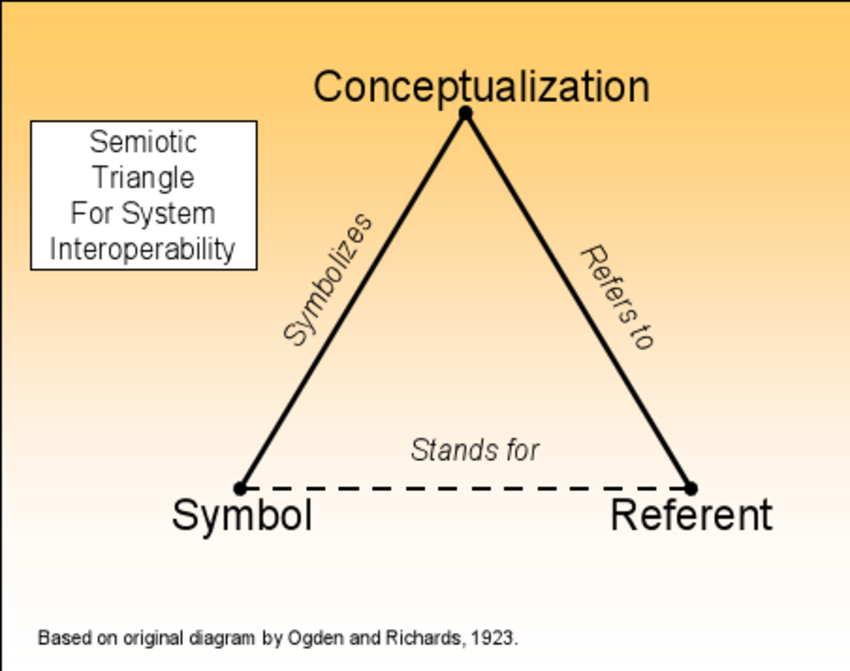
\includegraphics[width=\textwidth]{semiotic.png}}
\end{frame}

% \begin{frame}
%   \frametitle{Concepts, properties, relations}
%   \begin{itemize}
%   \item Non-relational concepts are sometimes called properties
%   \item Relational concepts are sometimes called (conceptual) relations
%   \end{itemize}
% \end{frame}

\begin{frame}
  \frametitle{What is an ontology?}
  \framesubtitle{Ontology: the philosophical discipline}
  \begin{itemize}
  \item Study of what there is (being {\em qua} being)
  \item reinterpreted for computer science: content {\em qua} content,
    independently of the way it is represented
  \item Study of the nature and structure of ``reality'' (a domain of discourse)
  \item A (philosophical) ontology: a structured system of entities assumed to exists,
    organized in categories and relations
  \end{itemize}
\end{frame}

\begin{frame}
  \frametitle{Aristotle's ontology}
  \centerline{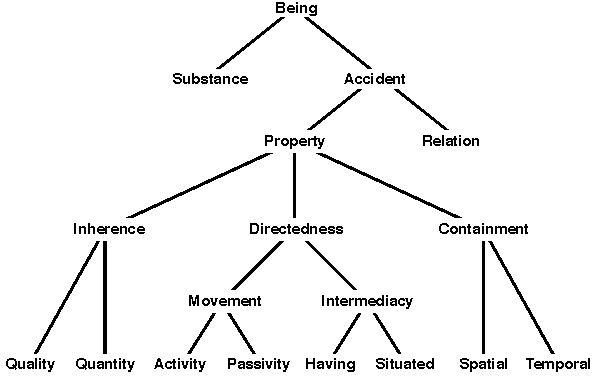
\includegraphics[width=\textwidth]{aristo.png}}
\end{frame}

\begin{frame}
  \frametitle{Ontologies in CS}
  \begin{itemize}
  \item Specific (theoretical or computational) artifacts expressing
    the intended meaning of a vocabulary in terms of primitive
    categories and relations describing the nature and structure of a
    domain of discourse 
    \begin{itemize}
    \item in order to account for the competent use of vocabulary in
      real situations
    \end{itemize}
  \end{itemize}
\end{frame}

\begin{frame}
  \frametitle{Ontologies in CS}
  \begin{itemize}
  \item Gruber: ``A specification of a conceptualization of a domain''
  \item Studer: ``An ontology is a formal, explicit specification of a
    shared conceptualization''
  \item Guarino: ``An ontology is a logical theory accounting for the
    intended meaning of a formal vocabulary, i.e. its ontological
    commitment to a particular conceptualization of the world. The
    intended models of a logical language using such a vocabulary are
    constrained by its ontological commitment. An ontology indirectly
    reflects this commitment (and the underlying conceptualization) by
    approximating these intended models.''
  \item Horrocks: ``an ontology [is] equivalent to a Description Logic
    knowledge base''
  \end{itemize}
\end{frame}

\begin{frame}
  \frametitle{What is a conceptualization}
  \begin{itemize}
  \item Formal structure of (a piece of) reality as perceived and organized by an
    agent, independently of:
    \begin{itemize}
    \item the vocabulary used
    \item the actual occurence of a specific situation
    \end{itemize}
  \item Different situations involving the same objects, described by
    different vocabularies, may share the same conceptualization
    \begin{itemize}
    \item Language 1: Apple
    \item Language 2: tafaha
    \end{itemize}
  \end{itemize}
\end{frame}

\begin{frame}
  \frametitle{Ontologies vs classifications}
  % Ontological analysis, slide 32
  \begin{itemize}
  \item Classifications focus on:
    \begin{itemize}
    \item access, based on pre-determined criteria (encoded by
      syntactic keys)
    \end{itemize}
  \item Ontologies focus on:
    \begin{itemize}
    \item meaning of terms
    \item nature and structure of a domain
    \end{itemize}
  \end{itemize}
\end{frame}

\begin{frame}
  \frametitle{Ontologies vs Knowledge bases}
  Knowledge base:
  \begin{itemize}
  \item Assertional component
    \begin{itemize}
    \item reflects specific states of affairs
    \item designed for problem solving
    \end{itemize}
  \item Terminological component (ontology)
    \begin{itemize}
    \item independent of states of affairs
    \item designed to support terminological services
    \item ... but independent of the actual terminology used
    \end{itemize}
  \item Ontological formulas are invariant, necessary information
    \begin{itemize}
    \item often expressed using Modal or Description Logics
    \end{itemize}
  \end{itemize}
\end{frame}

\begin{frame}
  \frametitle{Formal Ontology}
  Theory of formal distinctions and connections within
  \begin{itemize}
  \item entities of the world, as we perceive it (particulars)
  \item categories we use to talk about such entities (universals,
    concepts, properties)
  \end{itemize}
\end{frame}


\begin{frame}
  \frametitle{Ontologies}
  \begin{itemize}
  \item {\em classes} represent kinds of things in the world
    \begin{itemize}
    \item {\em Arm}, {\em Apoptosis}, {\em Influenza}, {\em Homo
        sapiens}, {\em Drinking behavior}, {\em Membrane}
    \end{itemize}
    \pause
  \item {\em instances} of classes are individuals satisfying the
    classes' intension
    \begin{itemize}
    \item my arm, the influenza I had last year, one ethanol molecule, etc.
    \end{itemize}
    \pause
  \item {\em relations} between instances arise from interactions,
    configurations, etc., of individuals
    \begin{itemize}
    \item my arm is {\bf part of} me, the {\bf duration of} my
      influenza was 10 days
    \item formal and material relations
    \end{itemize}
    \pause
  \item {\em axioms} specify our knowledge of the domain
    \begin{itemize}
    \item every instance of {\em Hand} is a {\bf part of} an instance
      of {\em Arm}
    \item $\forall x,y,z(Q(x) \land inheresIn(x,y) \land
      inheresIn(x,z) \rightarrow y=z)$
    \item $\forall x,y(\neg po(x,y) \rightarrow \exists z (po(z,y)
      \land \neg o(z,x)))$
    \end{itemize}
  \end{itemize}
\end{frame}

\begin{frame}
  \frametitle{The axiomatic method}
  The axiomatic method (Tarski) is a way to systematically
  identify and formalize a domain of knowledge
  \begin{enumerate}
  \item Identify the concepts in the domain; these constitute the
    signature $\Sigma$
  \item Reduce these concepts to primitive concepts through {\em
      explicit definitions}
  \item Find a set of statements that are true for the primitive terms
    within the domain of knowledge (axioms)
  \item Use a logical calculus to derive additional statements that
    are true within the domain
  \end{enumerate}
\end{frame}

\begin{frame}
  \frametitle{Ontologies in biology}
  \begin{itemize}
  \item Gene Ontology (1999)
    \begin{itemize}
    \item most widely used
    \item biological processes and cellular anatomy
    \end{itemize}
  \item Medical ontologies: UMLS, GALEN, SNOMED CT, ...
    \begin{itemize}
    \item not all are ``ontologies''
    \end{itemize}
  \end{itemize}
\end{frame}



% \begin{frame}
%   \frametitle{The formal tools of ontological analysis}
%   \begin{itemize}
%   \item Theory of Parts (Mereology)
%   \item Theory of Unity and Plurality
%   \item Theory of Essence and Identity
%   \item Theory of Dependence
%   \item Theory of Composition and Constitution
%   \item Theory of Properties and Qualities
%   \item Theory of Space and Time
%   \end{itemize}
% \end{frame}

% \begin{frame}
%   \frametitle{Top-level ontology}
%   \centerline{\includegraphics[width=.8\textwidth]{gfo-tree.pdf}}
% \end{frame}

% \begin{frame}
%   \frametitle{Top-level ontology}
%   \begin{itemize}
%   \item What does it mean to be a function?
%   \item What does it mean to be a {\em biological} function?
%   \item What is a material entity?
%   \item What is a cell?
%   \item What is a phenotype?
%   \end{itemize}
% \end{frame}



\end{document}
%%% Local Variables:
%%% mode: latex
%%% TeX-master: t
%%% End:
